\documentclass[a4paper]{article}
\usepackage[a4paper,%
    text={180mm, 260mm},%
    left=15mm, top=15mm]{geometry}
\usepackage[utf8]{inputenc}
\usepackage{cmap}
\usepackage[english, russian]{babel}
\usepackage{indentfirst}
\usepackage{amssymb}
\usepackage{amsmath}
\usepackage{mathtools}
\usepackage{tcolorbox}
\usepackage{romannum}
\usepackage{import}
\usepackage{xifthen}
\usepackage{pdfpages}
\usepackage{transparent}
\usepackage{graphicx}
\graphicspath{ {./figures} }

\newcommand{\incfig}[1]{%
\def\svgwidth{\columnwidth}
\import{./figures/}{#1.pdf_tex}
}

\begin{document}
\title{УМФ. Практика}
\author{Why am i even here?}
\maketitle
\section*{\centering Метод характеристик. Задача для бесконечной струны.}
\underline{Тип}\\
\begin{tcolorbox}
Записать формулы для закона движения точек струны и профиля струны\\
1) На Ox отмечаем точки где $ \phi(x) $ меняет свой вид\\
2) Через эти точки проводим характеристики\\
3) Записываем решение волнового уравнения. Делим фазовую плоскость на области 
записываем решение в каждой \\
4) Фиксируем t $ \rightarrow $  записываем решение как функцию от x\\
Фиксируем x $ \rightarrow $ записываем решение как функцию от t
\end{tcolorbox}

\begin{tcolorbox}
\underline{Пример}
\[
    u_{t t} - a^2 u_{xx}= 0
\]
\[
    u |_{t=0} = \phi(x) = 
    \begin{cases}
        \frac{h}{c} x + h &\quad x \in [-1, 0]\\
        -\frac{h}{c} x + h &\quad x \in [0, c]\\
        0 &\quad \text{иначе}\\
    \end{cases}
\]
\[
    u_t |_{t = 0} = 0
\]

Записать законы движения и тд
\end{tcolorbox}

\begin{figure}[!ht]
    \centering
    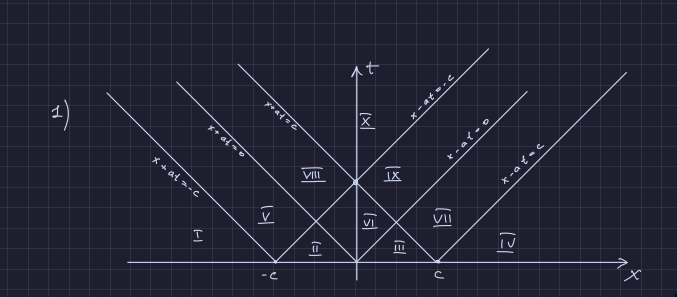
\includegraphics[width=0.95\textwidth]{mp-sem-pic1.png}
\end{figure}

\begin{figure}[!ht]
    \centering
    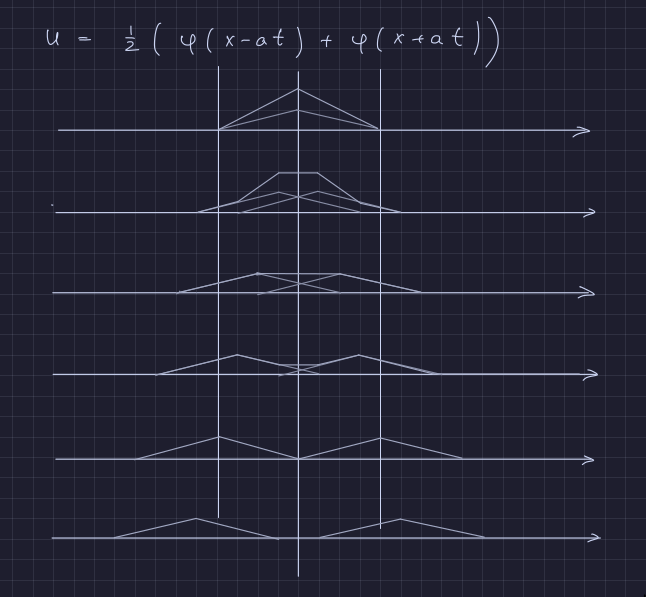
\includegraphics[width=0.90\textwidth]{mp-sem-pic2.png}
\end{figure}


\romannumeral 1 ) \[ u \equiv 0 \] \\

\romannumeral 2 ) \[ \begin{cases}
    -c < x - at < 0\\
    -c < x + at < 0\\
\end{cases} 
u = \frac{1}{2} (\frac{h}{c} (x + at) + h + \frac{h}{c} (x - at) + h) = \frac{h
}{c} x + h
\] 

\romannumeral 3 ) \[
    \begin{cases}
        0 < x + at < c\\
        0 < x - at < c\\
    \end{cases}
    u = -\frac{h}{c} + h
\]

\romannumeral 4 ) $ u \equiv 0 $ 

\romannumeral 5 ) 
\[
    \begin{cases}
        x - at < -c\\
        -c < x - at < 0\\
    \end{cases}
    u = \frac{1}{2} (\frac{h}{c} (x + at) + h)
\]

\romannumeral 6) 
\[
    \begin{cases}
        -c < x - at < 0\\
        0 < x + at < c
    \end{cases}
    u = \frac{1}{2} \left( \frac{h}{c} (x -at) + h - \frac{h}{c} (x + at) + h)
    \right) = -\frac{ah}{c} t + h
\]

\romannumeral 7)
\[
    \begin{cases}
        0 < x - at < c\\
        c < x + at
    \end{cases}
    u = \frac{1}{2} \left( -\frac{h}{c} (x - at) + h \right)
\]

\romannumeral 8)
\[
    \begin{cases}
        0 < x + at < c\\
        x - at < -c
    \end{cases}
    u = -\frac{1}{2} \left( -\frac{h}{c} (x + at) + h \right)
\]

\romannumeral 9)
\[
    \begin{cases}
        x + at > c\\
        -c < x - at < 0
    \end{cases}
    u = \frac{1}{2} \left( \frac{h}{c} (x -at) + h \right)
\]

\romannumeral 10)
\[
    \begin{cases}
        x + at > c\\
        x - at < -c
    \end{cases}
    u \equiv 0
\]

\begin{tcolorbox}
    \underline{Пример 2}
    \[
        \phi = \begin{cases}
            h \left( 1 - \frac{x^2}{c} \right) &\quad x \in [-c; c]\\
            0 &\quad x \notin [-c; c]
        \end{cases}
    \]
    \[
        \psi = 0
    \]
\end{tcolorbox}

\begin{figure}[!ht]
    \centering
    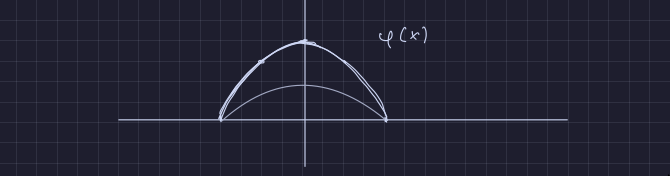
\includegraphics[width=0.8\textwidth]{mp-sem-pic3.png}
\end{figure}

\begin{figure}[!ht]
    \centering
    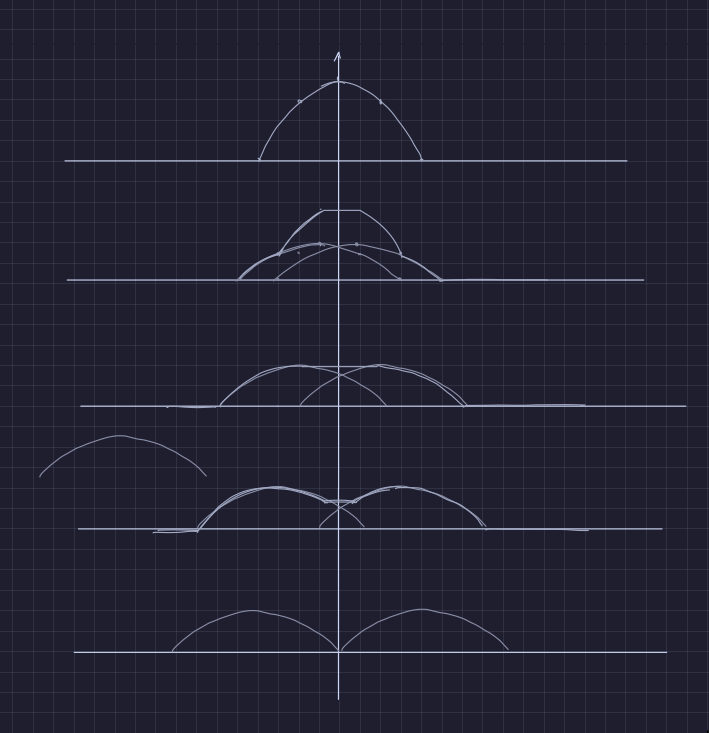
\includegraphics[width=0.8\textwidth]{mp-sem-pic4.png}
\end{figure}

\begin{figure}[!ht]
    \centering
    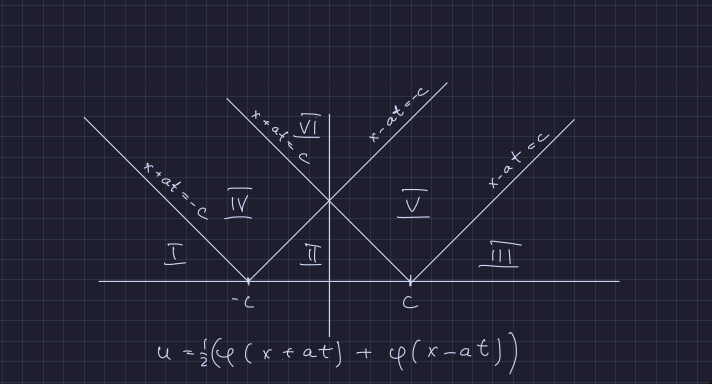
\includegraphics[width=0.8\textwidth]{mp-sem-pic5.png}
\end{figure}

\romannumeral 1)
\[
    \begin{cases}
        x + at < -c\\
        x - at < -c\\
    \end{cases}
    u = 0
\]

\romannumeral 2)
\[
    \begin{cases}
        -c < x + at < c\\
        -c < x - at < c\\
    \end{cases}
    u = \frac{1}{2} \left( h \left( 1 - \frac{(x + at)^2}{c^2} \right) + h
        \left( 1 - \frac{x - at)^2}{c^2} \right) \right) 
\]

\romannumeral 3)
\[
    \begin{cases}
        x - at > c\\
        x + at > c
    \end{cases}
    u = 0
\]

\romannumeral 4)
\[
    \begin{cases}
        -c < x + at < c\\
        x - at < -c
    \end{cases}
    u = \frac{1}{2} \left( h \left(1 - \frac{(x+at)^2}{c^2} \right) \right)
\]

\romannumeral 5)
\[
    \begin{cases}
        -c < x - at < c\\
        x + at > c
    \end{cases}
    u = \frac{1}{2} \left( h \left(1 - \frac{(x-at)^2}{c^2} \right) \right)
\]

\romannumeral 6)
\[
    \begin{cases}
        x + at > c\\
        x - at < -c
    \end{cases}
    u = 0
\]
\end{document}
